%!TEX root = ../../main.tex

\chapter{Technical Background and Related Works} \label{chap:background}
    \section{Introduction}
        This chapter provides the basic knowledge as well as related works regarding to the research topic of this thesis.
        Section \ref{sec:technical_background} introduces briefly the general architecture of deep neural networks for deep feature extraction; then describes in detail some dimensionality reduction algorithms and multi-view analysis algorithms.
        Section \ref{sec:related_works} summarizes approaches introduced in existing works to tackle problems in human action and gesture recognition and multi-view strategy.

    %!TEX root = ../../../main.tex

\section{Technical Background} \label{sec:technical_background}
    %!TEX root = ../../../main.tex

\subsection{Deep Neural Networks}
    \subsubsection{Artificial Neural Networks}
        Artificial neural networks (ANNs), sometimes a.k.a. multi-layer perceptron (MLP) or feed-forward neural network, are inspired by ``real'' neural networks - i.e. the human brain and nervous system.
        They consist of neurons grouped in multiple connected layers, each of which subsequently transformed by an activation function.

        \paragraph{Linear Layer}
            The \textit{linear layer}, or generally known as \textit{fully-connected layer}, basically composes of several perceptron units.
            Mathematically, it is simply a linear function of input features with 2 learnable parameters weight $W = \{\omega_1,\omega_2,...,\omega_d\}$ as coefficient of multiplication and bias $b$ as additional term, simulating the biological group of $d$ perceptrons:

            \begin{equation}
                y = W \cdot x + b
            \end{equation}

        \paragraph{Activation Layer}
            The non-linear \textit{activation layers} are responsible to create complex smooth mappings between the input and the output.
            They are element-wise operators responsible to squash the value of each element within the boundaries of specified function.
            Some common activation functions are:

            \begin{itemize}
                \item Sigmoid: $sigmoid\left(x\right) = \frac{1}{1 + e^{-x}}$
                \item Hyperbolic tangent: $tanh\left(x\right) = \frac{e^{x} - e^{-x}}{e^{x} + e^{-x}}$
                \item Rectifier: $relu\left(x\right) = \max\left(0, x\right)$
                \item Swish: $swish\left(x\right) = x \cdot sigmoid\left(x\right)$
            \end{itemize}

            For classification layer (the last linear layer), the number of neurons is equal to the number of classes to be recognized and a \textit{softmax} operator (Equation \eqref{eq:softmax}) is usually applied as activation function to get the probabilities of each classes.

            \begin{equation}
                \sigma_i = \frac{e^{y_i}}{\sum_{n=1}^{N}e^{y_n}}
                \label{eq:softmax}
            \end{equation}


        \paragraph{Training}
        Neural network training is usually performed via backpropagation algorithm.
        This algorithm is based on the calculation of a loss function $L$ which represents the difference between the network output and the expected output.
        Partial derivatives of the cost $\frac{\partial L}{\partial p_i}$ are calculated with regards to each trainable parameters $p_i$ using the chain rule.
        Then, each parameter is adjusted accordingly:

        \begin{equation}
            \Delta p_i = -\eta\frac{\partial L}{\partial p_i}
        \end{equation}

        where $\eta$ is called learning rate, which must be choosen carefully to ensure convergence.

        Loss functions are usually applied on the last layer.
        The most common criterion for classification tasks is \textit{Cross Entropy Loss}:

        \begin{equation}
            L_{CE} = -\frac{1}{N}\sum_{k=1}^{N}\log\frac{e^{W_{class(x_k)}x_k + b_{class(x_k)}}}{\sum_{i=1}^{c}e^{W_i x_k + b_i}}
        \end{equation}

        where $N$ is number of samples, $c$ is number of classes; $W$ and $b$ are parameters of classification layer, $W_i$ and $b_i$ denote the $i^{th}$ column of the weight $W$ and bias $b$ respectively; $x_k$ denotes the deep feature of $k^{th}$ sample belonging to the $class(x_k)$ class.

    \subsubsection{Convolutional Neural Networks}
        Convolutional neural networks (CNNs), inspired from the biological process in the visual cortex of animals, have emerged as the most efficient approach for image recognition and classification tasks.
        They are able to extract and aggregate highly abstract information from images and videos.
        As a result of huge research and engineering efforts, the effectiveness and performance of such algorithms have considerably improved, outperforming handcrafted methods for visual information embedding and becoming the state-of-the-art in image and video recognition.

        There are 5 main building blocks in architecture of a modern CNN:

        \paragraph{Convolution Layer}
            The \textit{convolutional layer} implements sliding kernel on the input tensor and for every position perform the summation of element-wise multiplication between sliced input and learnable weight matrices to compute the output.
            It can have multiple numbers of kernels such that more features from the input tensor can be extracted.

            The mathematical operation performed by each 2D convolutional kernel is:

            \begin{equation}
                o_{i,j}^l = \sum_{c=0}^{Ch}\sum_{h=0}^{K_H}\sum_{w=0}^{K_W}\left(\omega_{c,h,w}^l \cdot x_{c,i+h,j+w}\right) + b^l
            \end{equation}

            2D convolution is limited to spatial data and requires extra steps to manipulate temporarily continuous sequence of images.
            On the other hand, 3D convolution could intrinsically comprehend and establish abstract spatio-temporal relationship in 3D input tensor.
            The mathematical operation performed by each 3D convolutional kernel is:

            \begin{equation}
                o_{i,j,k}^l = \sum_{c=0}^{Ch}\sum_{d=0}^{K_D}\sum_{h=0}^{K_H}\sum_{w=0}^{K_W}\left(\omega_{c,d,h,w}^l \cdot x_{c,i+d,j+h,k+w}\right) + b^l
            \end{equation}

        \paragraph{Batch Normalization Layer}
            The \textit{batch normalization layer} introduced in \cite{ioffe2015batchnorm} is a pervasive component in modern CNN architectures.
            It generally escorts after every convolution layer and before an activation layer, responsible for bringing all the pre-activated features to the same scale.
            The mathematical equation is as follow:

            \begin{equation}
                y = \frac{x - \operatorname{E}[x]}{\sqrt{\operatorname{Var}[x] + \epsilon}} \cdot \gamma + \beta
            \end{equation}

            where $\operatorname{E}[x]$ and $\operatorname{Var}[x]$ stands for mean and standard deviation calculated per-dimension over the input mini-batches $x$; $\gamma$ and $\beta$ are learnable parameters and $\epsilon$ is a small number added to the denominator to ensure numerical stability.

        \paragraph{Activation Layer}
            Similar to activiation in ANNs, \textit{activation layer} in CNNs are element-wise operators that apply for each pixel of input tensor.

        \paragraph{Pooling Layer}
            The \textit{pooling layer} is usually inserted after one or a group of convolutional layers.
            The purpose of pooling is to progressively decrease the size of the elaborated data and make sure that only the most relevant features will be forwarded to the next layers.
            It follows the sliding kernel principle of convolution, but uses a much simpler operator without learnable parameter, such as:

            \begin{itemize}
                \item Max Pooling: Select the pixel with maximum value.
                \item Min Pooling: Select the pixel with minimum value.
                \item Average Pooling: Compute the mean of the sliced input pixels.
            \end{itemize}

            A special class of pooling layer is called \textit{global pooling}, which has flexible filter sizes and shifts exact to the shape of input tensor, squeezing each channel to a single scalar value.
            This type of pooling is generally used in the very end of a large-scale CNN, transforming high-level features of possibly unascertained shapes to a single vector of fixed length.
            After that, the output feature vector can be forwarded to further linear layers without being flattened or perform classification directly.

        \paragraph{Linear Layer}
            Similarly, \textit{linear layer} is the essential building block of classical ANNs, but might be optional in CNNs in case of fully convolutional neural networks.

    \subsubsection{Recurrent Neural Networks}
        A recurrent neural network (RNN) is a feed-forward neural network that takes previous time steps into account.
        The input of RNNs is a sequentially ordered collection of samples.
        Therefore, they excel in tasks in which order is important, e.g. time series forecasting, natural language processing.
        Relating to the research topic of this thesis, they can be used to handle chronical relationship of high-level representation of frames extracted from videos.

        In practice, either Long-Short-Term Memory (LSTM) or Gated Recurrent Unit (GRU) are used instead. 
        The main difference is that information that is deemed important is allowed to pass on to later time-steps without too much interference from hidden dot products and activation functions.

        \paragraph{Long Short-Term Memory}
        The LSTM architecture, contrary to regular RNNs, has an additional hidden state that is never directly outputted (see Figure \ref{fig:lstm_cell}). 
        This additional hidden state can then be used by the network solely for remembering previous relevant information. 
        Instead of having to share its ``memory'' with its output, these values are now separate. 
        During the training process, an LSTM learns what should be remembered for the future and what should be forgotten, which is achieved by using its internal weights.

        \begin{figure}[h!]
            \begin{center}
                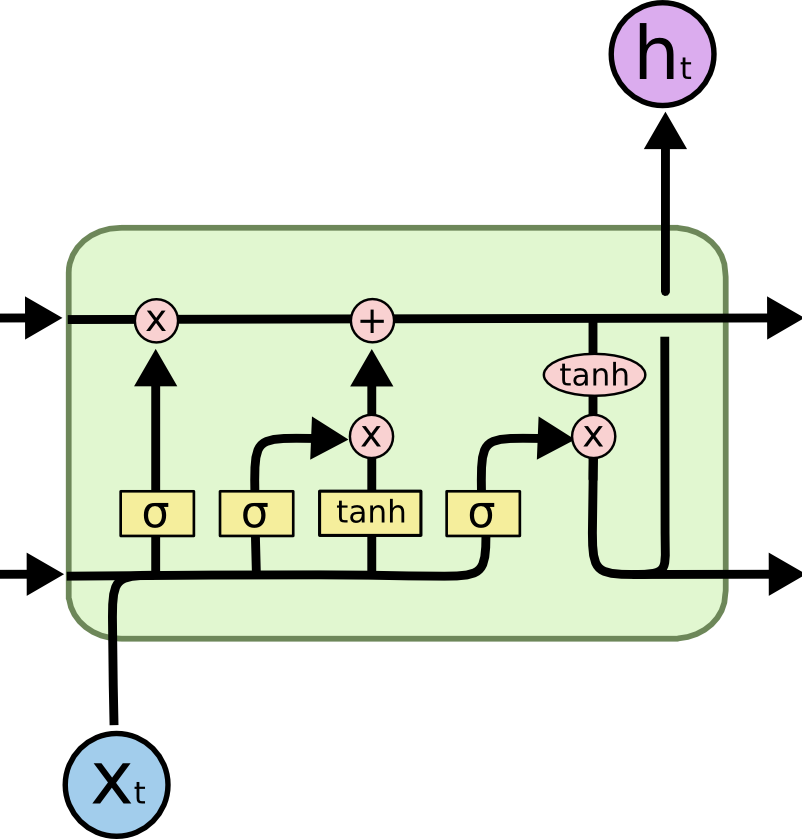
\includegraphics[scale=0.5]{figs/lstm_cell.png}
            \end{center}
            \caption{A single LSTM cell. From \cite{olah2015understanding}.}
            \label{fig:lstm_cell}
        \end{figure}

        As can be seen in the Figure \ref{fig:lstm_cell}, there are quite a few more parameters in this cell than in a normal RNN cell. 
        The calculation of the output vector and the hidden vector involves several operations.
        First of all the network determines how much of the hidden state to forget, also called the forget gate. 
        This is done by pushing both the previous iteration's output ($c_{t-1}$) and the forget gate vector ($f_t$) through a matrix multiplication, allowing the network to forget values at specific indices in the previous iteration's output vector. 
        $f_t$ can be obtained by using formula in Equation \eqref{eq:forget_vector_lstm}, where $W$ contains the weights for the input and $U$ contains the weights for the previous iteration's output vector, $x_t$ refers to the input, $h_{t-1}$ to the previous iteration's output vector and $b$ is bias:
        \begin{equation}
            f_t = \sigma(W_f x_t + U_f h_{t-1} + b_f)
            \label{eq:forget_vector_lstm}
        \end{equation}

        The network then determines what to remember from the input vector.
        This, commonly referred to as the input gate, is done by pushing the previous forget gate's output as well as the input gate through a matrix addition. 
        The output of the input gate ($i_t$) can be found by using the following formula:

        \begin{equation}
            i_t = \sigma(W_i x_t + U_i h_{t-1} + b_i)
            \label{eq:input_vector_lstm}
        \end{equation}

        The final hidden state vector ($c_t$) can then be found by using the previous two results as follows:

        \begin{equation}
            c_t = f_t \circ c_{t-1} + i_t \circ \sigma(W_c x_t + U_c h_{t-1} + b_c)
            \label{eq:hidden_state_vector_lstm}
        \end{equation}

        where $\circ$ denotes the Hadamard product (where each value at index $ij$ is the product of the values at the indices $ij$ in the two input matrices).
        This vector is then passed on to the next iteration. 
        Now the output gate vector $o_t$ and the output state $h_t$ can be optained:

        \begin{align} 
            o_t &= \sigma(W_o x_t + U_o h_{t-1} + b_o) \label{eq:output_gate_lstm}\\
            h_t &= o_t \circ \sigma(c_t) \label{eq:hidden_output_gate_lstm}
        \end{align}

        This results in a version of an RNN that is able to remember more and is more liberal in choosing what information it wants to keep in the hidden state and what it wants to discard. 
        This makes LSTM networks better suited for tasks involving series of data and become the predominant RNN architecture. 

        \paragraph{Gated Recurrent Units} Another RNN architecture is the GRU, introduced in \cite{cho2014learning}. 
        This architecture combines the input and forget gates into a single so-called ``update gate'' and also merges the cell state and hidden state (see Figure \ref{fig:gru_cell}). 
        The calculation of the merged output vector once again consists of several operations.
        The network first computes the ``reset gate'' $r_t$ using the following function, where $W_r$ are the weights for the reset gate and $[h_{t-1}, x_t]$ signifies the concatenation of $h_{t-1}$ and $x_t$:

        \begin{figure}[h!]
            \begin{center}
                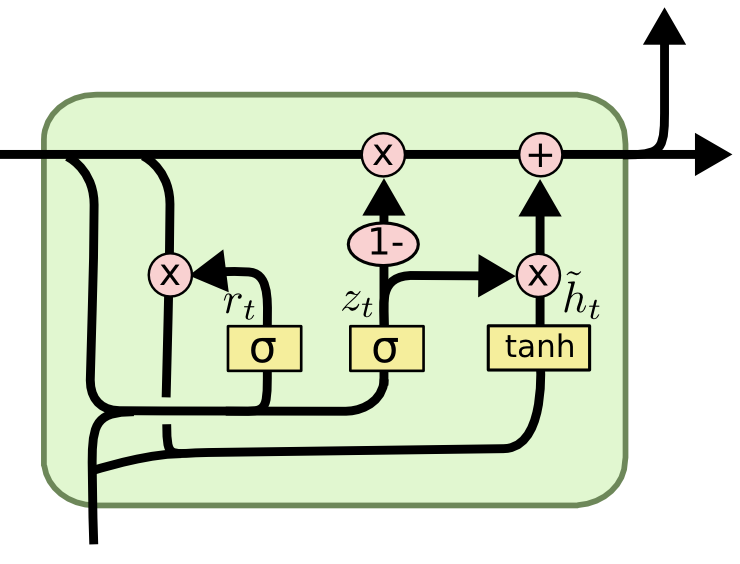
\includegraphics[scale=0.5]{figs/gru_cell.png}
            \end{center}
            \caption{A single GRU variation cell. From \cite{olah2015understanding}.}
            \label{fig:gru_cell}
        \end{figure}

        \begin{equation}
            r_t = \sigma\left(W_r [h_{t-1}, x_t]\right)
            \label{eq:gru_reset_gate}
        \end{equation}

        After this, the ``update gate'' $z_t$ is computed as follows, where $W_z$ holds the weights of the update gate:

        \begin{equation}
            z_t = \sigma\left(W_z [h_{t-1}, x_t]\right)
            \label{eq:gru_update_gate}
        \end{equation}

        The output vector $h_t$ (representing both the cell's output and its state) can then be computed by the following formula:

        \begin{equation}
            h_t = (1 - z_t) * h_{t-1} + z_t * \tilde{h_t}
            \label{eq:gru_output}
        \end{equation}

        where $\tilde{h_t} = \tanh(W * [r_t * h_{t-1}, x_t])$.

        % \paragraph{Bidirectional RNNs} It should be mentioned that when RNNs are used, they are often wrapped with a bidirectional layer.
        % This simply reverts the input sequence and enters the sequence in both the original and the reverse direction to two separate RNNs, usually LSTM or GRU.
        % % The usefulness of this is particularly intuitive when looking at the network in Figure \ref{fig:rnn}. 
        % When processing the entry $x^{(j)}$, only the entries $t < j$ are known. 
        % However, tokens later in the sequence might have an impact on the previous outputs of the model. 
        % Bidirectional RNNs are able to capture patterns that are overlooked by regular RNNs.

    %!TEX root = ../../main.tex

\subsection{Dimensionality Reduction Algorithms}
    Dimensionality reduction techniques are important in many applications related to machine learning.
    They aim to find low-dimensional embedding that should preserve sufficient information from the original dimension.
    Let's define $X = \{\boldsymbol{x}_{ik}|i=(1,..,c);k=(1,..,n_{i})\}$ as training samples where $\boldsymbol{x}_{ik} \in R^{d}$ is the $k^{th}$ sample of the $i^{th}$ class, $d$ is the original dimension of data, $m$ is the desired dimension of data after transformation such that $m < d$.

    \subsubsection{Linear discriminant analysis}
        The linear discriminant analysis (LDA) technique is developed to linearly transform the features into a lower dimensional space where the ratio of the between-class variance to the within-class variance is maximized, thereby guaranteering the optimal class separability.
        The projection results of $X$ on the lower dimensional space is denoted by $Y = \{\boldsymbol{y}_{ik} = w^T\boldsymbol{x}_{ik}|i=(1,..,c); k=(1,...,n_{i})\}$. $\boldsymbol{S}_B^y$ and $\boldsymbol{S}_W^y$ are computed as follows: 

        \begin{align}
            \boldsymbol{S}_W^y &= \sum_{i=1}^{c}\sum_{k=1}^{n_{i}}(y_{ik}-\boldsymbol{\mu}_i)(y_{ik}-\boldsymbol{\mu}_i)^T \label{eq:LDA_Sw_y}\\
            \boldsymbol{S}_B^y &= \sum_{i=1}^{c}n_i(\boldsymbol{\mu}_i - \boldsymbol{\mu})(\boldsymbol{\mu}_i - \boldsymbol{\mu})^T \label{eq:LDA_Sb_y}
        \end{align}

        where $\boldsymbol{\mu}_i=\frac{1}{n_i}{\sum_{k=1}^{n_{i}}}{\boldsymbol{y}_{ik}}$ is the mean of all samples of the $i^{th}$ class in the lower dimensional space; $\boldsymbol{\mu}=\frac{1}{n}\sum_{i=1}^{c}{\sum_{k=1}^{n_{i}}{\boldsymbol{y}_{ik}}}$ is the mean of all samples of all classes; $n=\sum_{i=1}^{c}n_i$ is the total number of data samples.
        The between-class $\boldsymbol{S}_B^y$ and within-class $\boldsymbol{S}_W^y$ covariance matrices in new dimension are not known yet but can be formulated as the linearly transformed versions of their counterparts $\boldsymbol{S}_B^x$ and $\boldsymbol{S}_W^x$ in original dimension.

        \begin{align}
            \boldsymbol{S}_W^y &= \omega^T\boldsymbol{S}_W^x\omega\\
            \boldsymbol{S}_B^y &= \omega^T\boldsymbol{S}_B^x\omega
        \end{align}

        $\boldsymbol{S}_B^x$ and $\boldsymbol{S}_W^x$ are easily calculable as follow:

        \begin{align}
            \boldsymbol{S}_W^x &= \sum_{i=1}^{c}\sum_{k=1}^{n_{i}}(x_{ik}-\boldsymbol{\mu}_i^{(x)})(x_{ik}-\boldsymbol{\mu}_i^{(x)})^T \label{eq:LDA_Sw_x}\\
            \boldsymbol{S}_B^x &= \sum_{i=1}^{c}n_i(\boldsymbol{\mu}_i^{(x)} - \boldsymbol{\mu}^{(x)})(\boldsymbol{\mu}_i^{(x)} - \boldsymbol{\mu}^{(x)})^T \label{eq:LDA_Sb_x}
        \end{align}

        Then the objective function is formulated by a Rayleigh quotient:

        \begin{equation}
            \boldsymbol{\omega}^* = \operatorname*{argmax}_{\boldsymbol{\omega}}\frac{trace(\boldsymbol{S}_B^y)}{trace(\boldsymbol{S}_W^y)} = \operatorname*{argmax}_{\boldsymbol{\omega}}\frac{trace(\omega^T\boldsymbol{S}_B^x\omega)}{trace(\omega^T\boldsymbol{S}_W^x\omega)}
            \label{eq:LDA}
        \end{equation}

        The Fisher's criterion in Equation \eqref{eq:LDA} can be reformulated as:

        \begin{equation}
            \boldsymbol{S}_W^x\omega = \lambda\boldsymbol{S}_B^x\omega
        \end{equation}

        where $\lambda$ represents the eigenvalues of the transformation matrix $\omega$. The analytical solution of $\boldsymbol{\omega}^*$ is optained by calculating the eigenvectors $V = \{v_1,v_2,...,v_m\}$ sorted by the scalar values of corresponding eigenvalues $\lambda = \{\lambda_1,\lambda_2,...,\lambda_m\}$ of the matrix $\boldsymbol{S} = {\boldsymbol{S}_W^x}^{-1}\boldsymbol{S}_B^x$.

    \subsubsection{Pairwise-covariance linear discriminant analysis}
        Pairwise-covariance linear discriminant analysis (pc-LDA) is an extension of LDA introduced in \cite{kong2014pairwise} that overcomes it's drawbacks by formulating pairwise distances between pairs of classes.
        The pairs of $a$ and $b$ classes are regarded as two Gaussian distributions $\mathcal{N}_a(\mu_a,{\boldsymbol{S}_W^y}_a), \mathcal{N}_b(\mu_b,{\boldsymbol{S}_W^y}_b)$ and the objective distance between two classes is defined as their Kullback-Leibler divergence \cite{kullback1951}:

        \begin{equation}
            D_{KL}\left(\mathcal{N}_a\parallel\mathcal{N}_b\right)=\frac{1}{2}\left(\mu_a-\mu_b\right)^{T}{\left({\boldsymbol{S}_W^y}_{ab}\right)}^{-1}\left(\mu_a-\mu_b\right),
        \end{equation}

        where ${\boldsymbol{S}_W^y}_{ab}$ is pairwise covariance matrix (Equation \eqref{eq:pc-LDA_Sw_ab}), calculated as the $\beta$ parameterized convex sum of global within-class scatter matrix $\boldsymbol{S}_W^y$ used in LDA with the within-class scatter matrix of each class ${\boldsymbol{S}_W^y}_i$ (Equation \eqref{eq:pc-LDA_Sw_i}).
        The author theorizes it would better represent the data distribution within two classes.

        \begin{align}
            {\boldsymbol{S}_W^y}_i &= \sum_{j=1}^{v}\sum_{k=1}^{n_{ij}}{\left(y_{ik}-\mu_i\right)\left(y_{ik}-\mu_i\right)^T} \label{eq:pc-LDA_Sw_i}\\
            {\boldsymbol{S}_W^y}_{ab} &= \beta\frac{n_a{\boldsymbol{S}_W^y}_a+n_b{\boldsymbol{S}_W^y}_b}{n_a+n_b}+\left(1-\beta\right){\boldsymbol{S}_W^y}
            \label{eq:pc-LDA_Sw_ab}
        \end{align}

        where $n_a$ and $n_b$ are number of samples belonging to class $a$ and $b$. The final objective is properly weighted to focus on classes with more samples:

        \begin{equation}
            \operatorname*{min}_{\boldsymbol{\omega}}{J}=\sum_{a=1}^{c}\sum_{b=a+1}^{c}{\frac{n_an_b}{{[2D_{KL}\left(\mathcal{N}_a\parallel\mathcal{N}_b\right)]}^q}},\ \ s.t.\ \omega^T\omega=\boldsymbol{I}
            \label{eq:pc-LDA}
        \end{equation}

        here $q\ge1$ is a hyper-parameter that controls how much the pairs of classes with smaller objective distances are biased over the others.

        The new model of pc-LDA is solved with a variant of gradient descent described in \cite{kong2014pairwise}, where $\nabla J\left(\omega\right)$ is computed and $\omega$ is updated as Equation \eqref{eq:pc-LDA_omega} in order to enforce $\omega$ on the Stiefel manifold. Every several iterations, due to numerical error, the learnt transformation is unitarized $\omega \leftarrow \omega{\left(\omega^T\omega\right)}^{-\frac{1}{2}}$ to ensure that the constraint $\omega^T\omega = \boldsymbol{I}$ is satisfied.

        \begin{equation}
            \omega \leftarrow \omega - \eta\left(\nabla J - \omega{[\nabla J]}^T\omega\right)
            \label{eq:pc-LDA_omega}
        \end{equation}

    %!TEX root = ../../../main.tex

\subsection{Multi-view Learning Algorithms}

    The motivation of multi-view learning (MvL) algorithms is to construct a common low-dimensional embedding that should preserve sufficient information or even be more informative than each individual view.

    Let's define $X = \{\boldsymbol{x}_{ijk}|i=(1,..,c);j = (1,..,v);k=(1,..,n_{ij})\}$ as samples from $v$ views where $\boldsymbol{x}_{ijk} \in R^{d_j}$ is the $k^{th}$ sample from the $j^{th}$ view of the $i^{th}$ class, $d_j$ is the dimensions of data at the $j^{th}$ view.
    Here ${\boldsymbol x}_{ijk}$ is a feature vector extracted from the $k^{th}$ sample from the $j^{th}$ view of the $i^{th}$ class.
    Different methods for features extraction from single view have been presented in previous sections. 

    \subsubsection{Multi-view discriminant analysis}
        Multi-view discriminant analysis (MvDA) is an extension of LDA for multi-view scenario \cite{kan2015multi}.
        It tries to determine a set of $v$ linear transformations to project all action samples from each view $j = (1,..,v)$ to a common space.
        The projection results of $X$ on the common space is denoted by $Y = \{\boldsymbol{y}_{ijk} = w_j^T\boldsymbol{x}_{ijk}|i=(1,..,c); j=(1,..,v); k=(1,...,n_{ij})\}$.
        The common space is built by maximizing the between-class variation $\boldsymbol{S}_B^y$ while minimizing the within-class variation $\boldsymbol{S}_W^y$ from all views. $\boldsymbol{S}_B^y$ and $\boldsymbol{S}_W^y$ are computed as follows: 

        \begin{align}
            \boldsymbol{S}_W^y &= \sum_{i=1}^{c}\sum_{j=1}^{v}\sum_{k=1}^{n_{ij}}(y_{ijk}-\boldsymbol{\mu}_i)(y_{ijk}-\boldsymbol{\mu}_i)^T \label{eq:MvDA_Sw}\\
            \boldsymbol{S}_B^y &= \sum_{i=1}^{c}n_i(\boldsymbol{\mu}_i - \boldsymbol{\mu})(\boldsymbol{\mu}_i - \boldsymbol{\mu})^T \label{eq:MvDA_Sb}
        \end{align}

        where $\boldsymbol{\mu}_i=\frac{1}{n_i}\sum_{j=1}^{v}{\sum_{k=1}^{n_{ij}}}{\boldsymbol{y}_{ijk}}$ is the mean of all samples of the $i^{th}$ class from all views in the common space; $\boldsymbol{\mu}=\frac{1}{n}\sum_{i=1}^{c}\sum_{j=1}^{v}{\sum_{k=1}^{n_{ij}}{\boldsymbol{y}_{ijk}}}$ is the mean of all samples of all classes from all views in the common space; $n=\sum_{i=1}^{c}n_i$ is the total data samples from all views.

        In order to separate the unknown transformation vectors, the between-class and within-class scatter matrices are reformulated as:

        \begin{align}
            \boldsymbol{S}_W^y &= W^{T}X\left(\boldsymbol{I} - \boldsymbol{E}\right)X^{T}W\\
            \boldsymbol{S}_B^y &= W^{T}X\left(\boldsymbol{E} - \frac{1}{n}\boldsymbol{\mathbbm{1}}\right)X^{T}W
        \end{align}
        where $W = \{\omega_1,\omega_2,...,\omega_v\}$ is concatenation of transformation vectors of all views; $\boldsymbol{I} \in \mathbb{R}^{n\times n}$ is identity matrix; $\boldsymbol{\mathbbm{1}} \in \mathbb{R}^{n\times n}$ is matrix of ones; $\boldsymbol{E} \in \mathbb{R}^{n\times n}$ is a square matrix whose elements satisfy:
        \begin{equation}
            \boldsymbol{E}_{kl} = \left\{\begin{array}{lr}
                \frac{1}{n_i}, & \text{if } class(x_k) = class(x_l) = i\\
                0, & \text{otherwise}
                \end{array}\right\}
        \end{equation}

        Then the objective function is formulated by a Rayleigh quotient:

        \begin{align}
            (\boldsymbol{\omega}_1^*,\boldsymbol{\omega}_2^*, ..., \boldsymbol{\omega}_v^*) &= \operatorname*{argmax}_{\boldsymbol{\omega}_1, \boldsymbol{\omega}_2,..., \boldsymbol{\omega}_v}\frac{trace({S}_B^y)}{trace({S}_W^y)}\\
            \boldsymbol{W}^* &= \operatorname*{argmax}_{\boldsymbol{W}}\frac{trace(W^{T}[X\left(\boldsymbol{E} - \frac{1}{n}\boldsymbol{\mathbbm{1}}\right)X^{T}]W)}{trace(W^{T}[X\left(\boldsymbol{I} - \boldsymbol{E}\right)X^{T}]W)}
            \label{eq:MvDA}
        \end{align}

        According to \cite{kan2016multi}, the problem satisfies the optimization form of generalized eigenvalue problem and could be analytically solved through eigenvalue decomposition.
        The concatenated $\boldsymbol{W}^* = \{\boldsymbol{\omega}_1^*,\boldsymbol{\omega}_2^*, ..., \boldsymbol{\omega}_v^*\}$ could be computed using the same procedure as $\boldsymbol{\omega}^*$ in LDA.
        Similarly, MvDA can be used as a dimensionality reduction algorithm by choosing $m$ eigenvectors corresponding to $m$ leading eigenvalues.

    \subsubsection{Multi-view discriminant analysis with view-consistency}

        In \cite{kan2016multi}, the authors observed that as multiple views correspond to the same objects, there should be some correspondence between multiple views.
        They then introduce a view consistency constraint into the objective function, that means if $X_j, X_r$ are observed at $j^{th}$ and $r^{th}$ views, there exists a certain transformation $\boldsymbol{R}$ such that $X_j = \boldsymbol{R}X_r$.
        As a result, the transformations obtained from two views (i.e. the projection of features extracted from singe view to common view) should have similar relationship: ${\omega}_j = \boldsymbol{R}{\omega}_r$.
        Let's define $\beta_i$ that captures the structure of the transformation ${\omega}_i$.

        \begin{equation}
            \omega_i = X_i\boldsymbol\beta_i
            \label{eq:MvDA-vc_beta}
        \end{equation}

        Then the $\beta_j$ and $\beta_r$ capturing the structures of two transformations of two views $j$ and $r$ should be identical ${\beta}_j = {\beta}_r$.

        Generalizing to $v$ views, suppose that ${\boldsymbol\beta}_j, j=(1,..,v)$ captures the structures of $v$ transformations ${w}_j$.
        Following the above observation, the $\boldsymbol{\beta}_r, r=(1,..,v)$ should resemble mutually.
        That means the similarity between the pair of $\boldsymbol{\beta}_j$ and $\boldsymbol{\beta}_r$ should be minimized. 

        \begin{equation}
            \sum_{j,r=1}^{v}||\boldsymbol{\beta_j} - \boldsymbol{\beta_r}||_2^2
            \label{eq:MvDA-vc_vc}
        \end{equation}

        From Equation \eqref{eq:MvDA-vc_beta}, we have:

        \begin{equation}
            \boldsymbol\beta_i = {\left(X_i^{T}X_i\right)}^{-1}X_i^{T}\omega_i \triangleq \boldsymbol{P}_iw_i
        \end{equation}

        Replacing in Equation \eqref{eq:MvDA-vc_vc} we can reformulate it as:

        \begin{equation}
            \sum_{j,r=1}^{v}||\boldsymbol{\beta_j} - \boldsymbol{\beta_r}||_2^2 = trace\left(W^{T}\boldsymbol{P}^{T}\left(2((v - 1)\boldsymbol{I} - \boldsymbol{\mathbbm{1}})\right)\boldsymbol{P}W\right)
        \end{equation}
        where $\boldsymbol{P} = \{\boldsymbol{P}_1,\boldsymbol{P}_2,...,\boldsymbol{P}_v\}$; $\boldsymbol{I} \in \mathbb{R}^{n\times n}$ is identity matrix; $\boldsymbol{\mathbbm{1}} \in \mathbb{R}^{n\times n}$ is matrix of ones.
        This term is called in \cite{kan2016multi} {\itshape view consistency} and will be added to the denominator of Equation \eqref{eq:MvDA}

        \begin{align}
            (\boldsymbol{\omega}_1^*,\boldsymbol{\omega}_2^*, ..., \boldsymbol{\omega}_v^*) &= \operatorname*{argmax}_{\boldsymbol{\omega}_1, \boldsymbol{\omega}_2,..., \boldsymbol{\omega}_v}\frac{trace({S}_B^y)}{trace({S}_W^y) + \alpha\sum_{j,r=1}^{v}||\boldsymbol{\beta_j} - \boldsymbol{\beta_r}||_2^2}\\
            \boldsymbol{W}^* &= \operatorname*{argmax}_{\boldsymbol{W}}\frac{trace(W^{T}[X\left(\boldsymbol{E} - \frac{1}{n}\boldsymbol{\mathbbm{1}}\right)X^{T}]W)}{trace(W^{T}[X\left(\boldsymbol{I} - \boldsymbol{E}\right)X^{T} + 2\alpha\boldsymbol{P}^T\left((v - 1)\boldsymbol{I} - \boldsymbol{\mathbbm{1}}\right)\boldsymbol{P}]W)}
            \label{eq:MvDA-vc}
        \end{align}

        This optimization problem could also be analytically solved by relaxing to the trace ratio optimization problem as Equation \eqref{eq:MvDA}.
        In the Equation \eqref{eq:MvDA-vc}, $\alpha$ is an empirically chosen parameter that puts a weight on the view-consistency assumption.
        When $\alpha = 0$, the MvDA-vc becomes the original MvDA. 


    %!TEX root = ../../main.tex

\section{Related Works} \label{sec:related_works}

    \subsection{Human action and gesture recognition}
        Action recognition has been an attractive research topic since the last decade \cite{zhang2019comprehensive}.
        Early methods represented human actions by extracting 2D/3D key-points such as Harris-3D, SIFT-3D, HOG-3DHOF \cite{laptev2008learning}, ESURF \cite{willems2008efficient} then computed a descriptor from the detected key-points.
        Action representation  by a set of key-points could loose the temporal information. Therefore, Wang and Schmid in \cite{wang2013action} proposed a feature named improved dense trajectories (iDT) that densely sample and track optical flow points along trajectories.
        iDT has become state-of-the-art hand-crafted features and widely used for many video-based tasks.
        However, when working with large-scale datasets, iDT becomes intractable on due to its expensive computational cost and poor performance. 

        To work with more challenging datasets, effective action recognition approaches rely on powerful learning methods, particularly the deep learning techniques.
        Early works applied 2D CNN on frames of video sequence and then aggregated the information using pooling techniques \cite{karpathy2014large}.
        To exploit the temporal information, different architectures such as LSTM with the internal mechanisms called gates that can deal with short-term memory are proposed \cite{sun2017lattice}.
        Recently, instead of using 2D convolutional operators, different 3D CNN have been proposed \cite{ji20123d, tran2015learning, varol2017long}.
        Besides, to boost the recognition performance, different approaches tried to combine multiple streams \cite{wang2015towards, feichtenhofer2016convolutional, khong2018improving} or to combine both multiple features \cite{wang2015action, christoph2016spatiotemporal}. %trajectory-pooled deep-convolutional
        %descriptor - TDD;  ST-ResNet+iDT
        %Recently, many other architectures such as temporal Segment Networks - TSN \cite{wang2016temporal}, ST-VLMPF \cite{duta2017spatio}, P3D ResNet \cite{qiu2017learning}, I3D\cite{carreira2017quo}, 3D ResNeXt \cite{hara2018can}, R(2+1) D-TwoStream \cite{tran2018closer}, CO2FI+ASYN \cite{lin2018action}, and DML \cite{chen2017deep} have shown state-of-the-art performances in action recognition.
        %Previous section briefly gives a survey of different techniques for features extraction and action recognition from common views.

        These aforementioned approaches focus on single view action recognition, cross-view action recognition is more challenging and requires additional techniques to be taken into account. 
        Junejo et al. in \cite{junejo2008cross} proposed a descriptor, namely self-similarity matrix (SSM), which is an exhaustive table of distances between image features taken by pair from the image sequences.
        Liu et al. \cite{liu2011cross} employed cuboids extracted from each video and BoW model to build video descriptor for each single view. Then, a bipartite graph is built to model two view-dependent vocabularies.
        Li et al. \cite{li2012discriminative} described each video by concatenating spatio-temporal interest-point-based descriptor with shape flow descriptor. Then, to deal with cross-view, they construct ‘virtual views’, each is a linear transformation between action descriptors from one viewpoint and those from another.
        The method in \cite{zheng2012cross, zheng2013learning} employed the same video representation manner as in \cite{li2012discriminative}.
        However, a transferable dictionary between source and target view has been learnt to force features of the same action extracted from two views having the same sparse representation. 
        %In \cite{ulhaq2017space}, the authors proposed an advanced space-time filtering framework for recognizing human actions despite large viewpoint variations. Specifically, they used 3D tensor structure at each pixel, which characterizes the most common local motion in action sequences. Discrete tensor Fourier transform is then applied to achieve frequency domain representations. Then, they form view clusters from multiple-view action data and use space-time correlation filtering to achieve robust view representations. 

        Previous cross-view action recognition techniques usually connect source and target views with a set of linear transformations, that are unable to capture the non-linear manifolds on which real actions lie. In \cite{rahmani2017learning}, the authors find a shared high-level non-linear virtual path that connects multiple source and target views to the same canonical view. This virtual path is learnt by a deep neural network. In \cite{kong2017deeply}, a deep learning technique that stacks multiple layers of feature learners is designed to incorporate both private and shared view features. 
        In \cite{liu2018hierarchically}, the authors concatenated both private and shared view features and learnt transferable dictionary pair from a pair of views. In \cite{zhang2018action}, the authors proposed a framework to jointly learn a a view-invariant transfer dictionary and a view-invariant classifier using synthetic data during the pre-training phase to extract view-invariance between 3D and 2D videos.

        %As we have analyzed, multi-view  analysis has been actively studied. Several innovative ideas have been proposed. As a result, performance of multi-view classification is significantly improved. However, most of these methods are experimented on still images. The question of how still good those methods a special time-series data (i.e. video data) has been not addressed. In this paper, we contribute to improve the model of common feature space. In addition, we will evaluate the proposed method on video data, where both temporal and spatial features must be taken into account.

    \subsection{Multi-view analysis and learning techniques}
        As many objects in the real-world can be observed from different viewpoints, to exploit the consensual and complementary information between different views, Multi-view analysis (MvA) techniques are employed.
        MvA is a strategy for fusing data from different sources or subsets.

        Canonical Correlation Analysis (CCA) \cite{Hotelling} can be considered as the first approach of MvL with the aim to find pairs of projections for two views so that the correlations between these views are maximized.
        As CCA can only handle the linear correlation, Kernel CCA (KCCA) was proposed to take non-linear correlation relationship of data into account \cite{Akaho2006}.
        However, both CCA and KCCA are unsupervised methods and can not leverage the label information.
        In \cite{diethe2008multiview}, a supervised approach named Multi-view Fisher discriminant analysis (MvFDA) was proposed for binary classification problem.
        All of aforementioned methods are only applicable for two views problem.

        To extend to multiple view cases, a natural extension is to maximize the sum of the pairwise correlations.
        In a general case, it would be better to build a common shared feature space that captures latent information of the object from all observed views.
        For this propose, Multi-view CCA (MvCCA) is proposed in 2010 to build a common feature space of all views \cite{rupnik2010multi}. 
        %MCCA tried to find $v$ transformations by maximizing the correlation of every two views. 
        However, MvCCA did not consider the discrepancy information but only maximizing the correlation between every two views, so that it may be ineffective for classification across views. 
        %Generalized Multi-view Analysis (GMA) preserves the supervised structure of each view while keeping the projections of different views close to each other in the latent common space. GMA is considered as an extension of Fisher Discriminant analysis (FDA) for cross-view problem. It considers class label information so it could be good for multi-view classification. However, GMA considers only the the discriminant information in each individual view, not inter-view so it could decrease cross-view recognition.
        %Multi-view Uncorrelated Linear Discriminant Analysis (MULDA) \cite{sun2015multi-view} learnt uncorrelated discriminant features by using Uncorrelated Linear Discriminant Analysis (ULDA). Multi-view Modular Discriminant Analysis (MvMDA) \cite{cao2017generalized} was proposed to separate class centers across different views. 

        In \cite{kan2015multi}, Multi-view discriminant analysis (MvDA), an extension of linear discriminant analysis (LDA) for multi-view problem was proposed.
        MvDA tries to optimize jointly view correlation, intra-view and inter-view discriminability. 
        An extension of MvDA which considers view-consistency was also introduced and achieved significant performance improvement.

        In \cite{zhao2018multi}, the authors proposed multi-view manifold learning with locality alignment (MvML-LA) framework to realize manifold learning under multi-view scenario. 
        %Locality alignment in the latent space learning is considered to enhance its discriminative capability and developed two specific algorithms in supervised and unsupervised scenarios, respectively. 

        Most recently, \cite{you2019multi} proposed Multi-view Common Component Discriminant Analysis (MvCCDA) technique that both integrates supervised information and local geometric information into the common component extraction process.
        This helps to effectively handle view discrepancy, discriminability and non-linearity in a joint manner.


    \section{Summary}
        In this chapter, various related works were briefed.
        The general concepts of deep neural networks, especially 3D CNN because of its outstanding performance in action recognition for video data, are explained.
        Also, the underlying mathematical model behind LDA and two utilized multi-view analysis algorithms inspired by it (MvDA \& MvDA-vc) were clarified.
        In addition, an extension of LDA called pc-LDA that enhances it with better class discrepancy constraints were introduced.
